\clearpage
\section{Empirical Study}\label{sec:empirical}

\subsection{Institutional setting, source audit, and analysis sample}
The empirical application re-examines the 18 February--1 March 2020 police strike in Cear\'a studied by \cite{mancha2025}. The primary source is the 27,830 victim records in \texttt{Painel.xlsx}; \texttt{Gang\_Turfs.xlsx} supplies the gang-exposure measure. The released \texttt{Daily\_Homicides\_CE.dta} is an intermediate aggregation of the victim records, not independent evidence. We reconstruct its outcomes from the spreadsheet and compare unit--day totals after identical AIS and municipality normalization. The intermediate file has one duplicated unit--day; after re-aggregation its 27,418 valid-AIS homicides and all unit--day outcome counts agree with the source reconstruction. Seven exact duplicate source rows are retained because the data are victim records and the source does not establish that they are duplicate victims.

We exclude 412 records with absent or non-geographic AIS labels, retain 358 municipality/district units in 22 AIS, and balance every unit over 2,557 dates (1 January 2014--31 December 2020). Of 915,406 unit--days, 893,515 have no recorded homicide and are filled with zero. The main 97-day window has 34,726 unit--days (33,943 zero), 989 victim records, 94 treated units and 264 controls. The seven outcomes are total homicides, men, women, and the released \texttt{crime\_1}--\texttt{crime\_4} indicators, all as unit--day counts. To reproduce the released Stata coding, women equal total minus men; 24 records with unclassified sex therefore enter this residual category. This is a measurement limitation, not an assertion that their victims were female. The original spreadsheet, intermediate file, source-code hash, row flow, and discrepancy checks are preserved in the accompanying reproduction archive.

The primary treated set is AIS 02, 06, 11, 12, and 13, matching the paper's stated five high-exposure areas. The released Stata code lowercases AIS labels and later tests the uppercase literal \texttt{AIS 13}; that test fails, making its executed treated set AIS 02, 06, 11, and 12. We use this four-AIS version only as a replication and sensitivity case. A separate boundary issue arises from the 75th percentile of \texttt{ExposureDistricts}: its value is 0.587728, whereas AIS 07 is 0.588235. A mechanical ``greater than percentile'' rule includes AIS 07 and yields six areas. We report that six-AIS case separately rather than silently redefine the paper's intended five areas.

\subsection{Common TWFE benchmark and gap correction}
The analysis window consists of the 84 days ending 17 February 2020 and the 13 strike days. Each municipality/district receives equal weight within its treatment arm. The common benchmark is the coefficient on $D_i\times S_t$ in
\begin{equation}\label{eq:empiricaltwfe}
Y_{it}=\alpha_i+\lambda_t+\tau^{\mathrm{TWFE}}D_iS_t+u_{it},
\end{equation}
where $\alpha_i$ and $\lambda_t$ are unit and date effects. With the balanced panel and one common treatment date, direct two-way residualization verifies that this coefficient equals the post-strike treated-minus-control gap less the pre-strike mean gap for all seven outcomes; the largest numerical discrepancy is $6.8\times10^{-15}$.

Let $G_t$ denote that daily unit-weighted group gap. For each candidate $m$ we use the \emph{same} $\widehat\tau^{\mathrm{TWFE}}$ and pre-period baseline:
\begin{equation}\label{eq:empiricalbias}
\widehat B_m=\overline{\widehat G^{0}_{m,\mathrm{post}}}-\overline G_{\mathrm{pre}},\qquad
\widehat\tau_m=\widehat\tau^{\mathrm{TWFE}}-\widehat B_m
=\overline G_{\mathrm{post}}-\overline{\widehat G^{0}_{m,\mathrm{post}}}.
\end{equation}
Every forecast is averaged over seven days in the first strike block and six in the second, equivalently weighting the two block means by $7/13$ and $6/13$. The no-correction forecast sets $\overline{\widehat G^{0}}=\overline G_{\mathrm{pre}}$. The linear-gap method fits an ordinary line to twelve pre-strike weekly gap means and extrapolates weeks 13 and 14. Synthetic Control matches the treated arm's single 84-day pre-mean with nonnegative control-unit donor weights summing to one, then uses contemporaneous donor outcomes to forecast the treated mean and subtracts the contemporaneous unweighted control mean. Because a single matching predictor leaves many exact solutions, this implementation uses a maximum-entropy tie-break based on donor multiplicity; it is a transparent empirical implementation of the simulation's one-predictor design, not a claim to reproduce every numerical detail of the original \texttt{Synth} solver.

The Random Forest and Gradient Boosting retain the simulation's tree counts and major tuning choices (500 trees and two candidate features per forest split; 800 depth-three boosting trees, learning rate 0.01, leaf size ten, subsample 0.7). Their empirical prediction target is different. The simulated $X_1,X_2,X_3$ do not exist in these data, so each model fits the two daily \emph{group mean} series, using only relative day, treatment-arm label, weekday and calendar month. It predicts both group means and takes their difference. Relative day, weekday, month, and arm label are known at forecast time. Models are refitted inside each window. Synthetic Control may use contemporaneous control outcomes; no candidate uses strike-period treated outcomes to fit or select its counterfactual. Forest and boosting forecasts beyond the training dates should not be interpreted as unrestricted extrapolation of a latent trend: terminal-tree predictions are bounded by training responses.

\subsection{Pre-strike evaluation and selection}
The true untreated strike-period gap is unobserved, so empirical ATT bias cannot be measured. We instead run the same 84-day training/13-day testing exercise at 154 pre-strike origins, moving the origin by 14 days each time. Each origin re-estimates all five candidates and treats the ensuing 13 days as a zero-effect placebo. The resulting pseudo-effect is $\overline G_{\mathrm{test}}-\overline{\widehat G^0_{m,\mathrm{test}}}$, algebraically the common placebo TWFE less the candidate's predicted bias term. We report mean signed error, population variance, MAE, RMSE, available windows, and failures. The winner for each outcome is fixed by the smallest pre-strike placebo RMSE, with no inspection of strike outcomes. The 13-day test blocks do not overlap at a 14-day step, but adjacent 84-day training blocks do; paired window differences are correlated and a naive window-level standard error is not an independent-sample uncertainty measure.

\begin{table}[htbp]
\centering\small
\caption{Total-homicide rolling pre-strike placebo performance (154 windows, 84-day training and 13-day test). The pseudo-effect is zero; variance is the population variance of placebo estimates. SC--entropy uses an entropy tie-break; RF--empirical and GB--empirical use forecast-known calendar and group features.}
\label{tab:placeborebuild}
\begin{tabular}{lrrrrrr}
\toprule
Method & Signed error & Variance & MAE & RMSE & Windows & Failures\\
\midrule
No correction & 0.00028 & 0.000069 & 0.00675 & 0.00830 & 154 & 0\\
Linear gap & -0.00008 & 0.000090 & 0.00755 & 0.00946 & 154 & 0\\
SC--entropy & 0.00105 & 0.000076 & 0.00718 & 0.00876 & 154 & 0\\
RF--empirical & 0.00202 & 0.000061 & 0.00642 & 0.00809 & 154 & 0\\
GB--empirical & 0.00018 & 0.000067 & 0.00655 & 0.00820 & 154 & 0\\
\bottomrule
\end{tabular}
\end{table}


For total homicides, Random Forest has the smallest pre-strike RMSE (0.00809), versus 0.00830 for no correction, 0.00820 for Gradient Boosting, 0.00876 for Synthetic Control, and 0.00946 for the linear gap. Its 2.6\% advantage over unadjusted TWFE is modest, and it has a positive mean signed placebo error (0.00202), so this ranking is evidence of relative pre-period prediction, not proof that strike-period selection bias was eliminated. A lag-six HAC sensitivity for the paired forest-versus-TWFE MSE difference gives $-3.49\times10^{-6}$ with a standard error of $6.42\times10^{-6}$; it does not resolve the close ranking statistically. Random Forest also ranks first for men, women and three of the four crime indicators; no correction ranks first for \texttt{crime\_4}. The full all-outcome performance table is in Table~\ref{tab:allplaceborebuild} below.

\begin{figure}[htbp]\centering
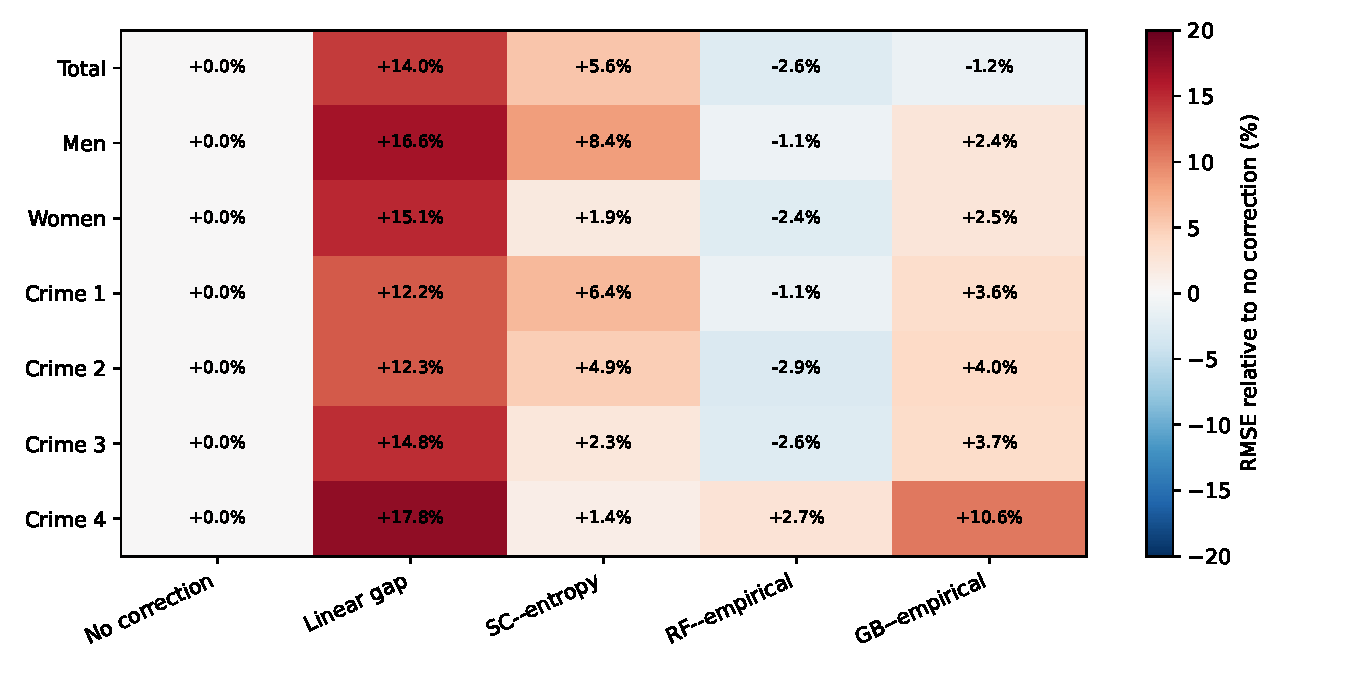
\includegraphics[width=0.88\linewidth]{figures/empirical_rmse_rebuild.pdf}
\caption{Pre-strike placebo RMSE relative to no correction; negative values indicate lower RMSE. All comparisons use the same 154 rolling windows.}\label{fig:empiricalrmserebuild}
\end{figure}

\subsection{Strike-period estimates and AIS resampling}
After the selection rule is frozen, all five methods are refitted on the actual 84 pre-strike days, and every pre-specified estimate is reported. For total homicides the common TWFE DID is 0.03437 per municipality/district-day. The linear, Synthetic Control, Random Forest, and Gradient Boosting predicted bias terms are respectively 0.00732, 0.04560, $-0.00169$, and $-0.00136$, giving adjusted estimates 0.02705, $-0.01123$, 0.03606, and 0.03573. Synthetic Control's larger downward adjustment reflects its donor-based forecast of a higher untreated strike-period gap; its information set differs because the control outcomes are contemporaneous. It was not selected by the pre-strike rule. Table~\ref{tab:estimatesrebuild} gives every outcome, the identical within-outcome TWFE, its candidate-specific bias term, corrected estimate and fixed-method interval.

\begin{longtable}{llrrrrl}
\caption{Strike-period TWFE, predicted bias and correction on the common unit/date panel. Percentile intervals resample AIS within treatment arms; * marks the pre-strike RMSE winner.}\label{tab:estimatesrebuild}\\
\toprule
Outcome & Method & TWFE & Bias $\widehat B_m$ & Adjusted & 95\% interval & Selected\\
\midrule
\endfirsthead
\toprule
Outcome & Method & TWFE & Bias & Adjusted & 95\% interval & Selected\\
\midrule
\endhead
Total & No correction & 0.0344 & 0.0000 & 0.0344 & [-0.016, 0.142] & \\
Total & Linear gap & 0.0344 & 0.0073 & 0.0271 & [-0.018, 0.135] & \\
Total & SC--entropy & 0.0344 & 0.0456 & -0.0112 & [-0.045, 0.065] & \\
Total & RF--empirical & 0.0344 & -0.0017 & 0.0361 & [-0.013, 0.155] & *\\
Total & GB--empirical & 0.0344 & -0.0014 & 0.0357 & [-0.012, 0.156] & \\
\midrule
Men & No correction & 0.0320 & 0.0000 & 0.0320 & [-0.015, 0.144] & \\
Men & Linear gap & 0.0320 & 0.0062 & 0.0257 & [-0.017, 0.135] & \\
Men & SC--entropy & 0.0320 & 0.0416 & -0.0096 & [-0.039, 0.067] & \\
Men & RF--empirical & 0.0320 & -0.0045 & 0.0365 & [-0.008, 0.152] & *\\
Men & GB--empirical & 0.0320 & -0.0052 & 0.0372 & [-0.007, 0.153] & \\
\midrule
Women & No correction & 0.0024 & 0.0000 & 0.0024 & [-0.007, 0.011] & \\
Women & Linear gap & 0.0024 & 0.0011 & 0.0013 & [-0.009, 0.011] & \\
Women & SC--entropy & 0.0024 & -0.0012 & 0.0036 & [-0.008, 0.012] & \\
Women & RF--empirical & 0.0024 & 0.0008 & 0.0016 & [-0.007, 0.012] & *\\
Women & GB--empirical & 0.0024 & 0.0027 & -0.0003 & [-0.010, 0.010] & \\
\midrule
Crime 1 & No correction & 0.0214 & 0.0000 & 0.0214 & [-0.006, 0.076] & \\
Crime 1 & Linear gap & 0.0214 & 0.0020 & 0.0195 & [-0.007, 0.075] & \\
Crime 1 & SC--entropy & 0.0214 & 0.0186 & 0.0028 & [-0.020, 0.051] & \\
Crime 1 & RF--empirical & 0.0214 & -0.0048 & 0.0262 & [-0.002, 0.081] & *\\
Crime 1 & GB--empirical & 0.0214 & -0.0044 & 0.0258 & [-0.002, 0.082] & \\
\midrule
Crime 2 & No correction & 0.0178 & 0.0000 & 0.0178 & [-0.008, 0.067] & \\
Crime 2 & Linear gap & 0.0178 & 0.0026 & 0.0152 & [-0.009, 0.064] & \\
Crime 2 & SC--entropy & 0.0178 & 0.0163 & 0.0015 & [-0.021, 0.045] & \\
Crime 2 & RF--empirical & 0.0178 & -0.0031 & 0.0209 & [-0.005, 0.070] & *\\
Crime 2 & GB--empirical & 0.0178 & -0.0026 & 0.0205 & [-0.004, 0.069] & \\
\midrule
Crime 3 & No correction & 0.0120 & 0.0000 & 0.0120 & [-0.010, 0.051] & \\
Crime 3 & Linear gap & 0.0120 & 0.0032 & 0.0088 & [-0.013, 0.044] & \\
Crime 3 & SC--entropy & 0.0120 & 0.0122 & -0.0002 & [-0.022, 0.034] & \\
Crime 3 & RF--empirical & 0.0120 & -0.0024 & 0.0144 & [-0.006, 0.051] & *\\
Crime 3 & GB--empirical & 0.0120 & -0.0028 & 0.0148 & [-0.005, 0.052] & \\
\midrule
Crime 4 & No correction & 0.0094 & 0.0000 & 0.0094 & [-0.012, 0.047] & *\\
Crime 4 & Linear gap & 0.0094 & 0.0030 & 0.0063 & [-0.015, 0.046] & \\
Crime 4 & SC--entropy & 0.0094 & 0.0094 & -0.0000 & [-0.021, 0.038] & \\
Crime 4 & RF--empirical & 0.0094 & -0.0016 & 0.0110 & [-0.010, 0.050] & \\
Crime 4 & GB--empirical & 0.0094 & -0.0014 & 0.0108 & [-0.010, 0.049] & \\
\bottomrule
\end{longtable}


For fixed-method uncertainty we resample AIS, with replacement separately among five treated and seventeen control clusters, and refit the final 84/13-day calculation on each draw. Percentile intervals summarize 499 draws for each of 35 outcome--method estimates. The selected total-homicide Random Forest interval is $[-0.0126,0.1552]$, and none of the seven selected fixed-method intervals excludes zero. For total homicides we additionally repeat the \emph{entire} 154-window model-selection exercise inside each of 99 AIS draws, then refit that draw's selected method in the strike window. The re-selection result is reported separately from fixed-method intervals. Only five treated AIS are available, so neither percentile construction nor model re-selection removes substantial few-cluster uncertainty; the 99-draw selection-aware interval in particular has coarse tail resolution. AIS resampling also assumes that these clusters are a meaningful basis for uncertainty, not that treatment is randomized across them.

\begin{table}[htbp]
\centering\small
\caption{Fixed-method versus full selection-aware AIS bootstrap for total homicides. Both rows share the original-sample point estimate; percentile intervals differ in whether selection is repeated.}
\label{tab:selectionrebuild}
\begin{tabular}{lrrrl}
\toprule
Procedure & Draws & Estimate & 95\% interval & Re-selection\\
\midrule
Random Forest fixed & 499 & 0.0361 & [-0.0126, 0.1552] & No\\
Full RMSE selection & 99 & 0.0361 & [-0.0254, 0.1433] & Yes\\
\bottomrule
\end{tabular}
\end{table}

Across 99 selection-aware resamples, the pre-strike RMSE rule chose no correction 61, linear gap 0, Synthetic Control 19, Random Forest 15, Gradient Boosting 4. The observed-sample winner was Random Forest. Selection changes across draws, showing that the small placebo-RMSE advantage is sensitive to AIS composition. Neither interval is a randomization-based causal interval.


\begin{figure}[htbp]\centering
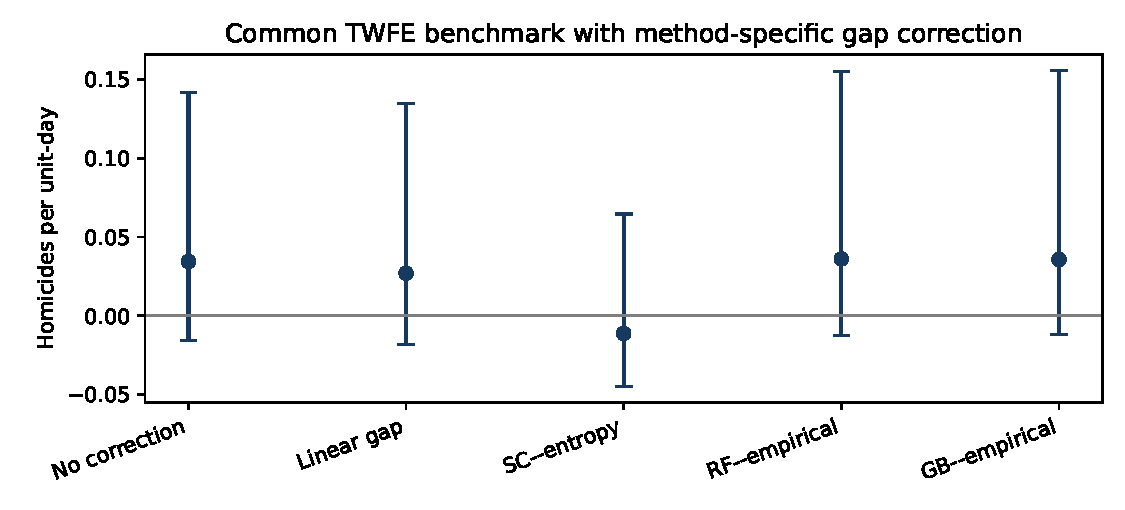
\includegraphics[width=0.82\linewidth]{figures/empirical_total_estimates_rebuild.pdf}
\caption{Total-homicide estimates and fixed-method 95\% AIS-bootstrap percentile intervals, all aligned to the same TWFE benchmark. The displayed intervals do not repeat model selection; Table~\ref{tab:selectionrebuild} gives the selection-aware comparison.}\label{fig:totalestimatesrebuild}
\end{figure}

\begin{figure}[htbp]\centering
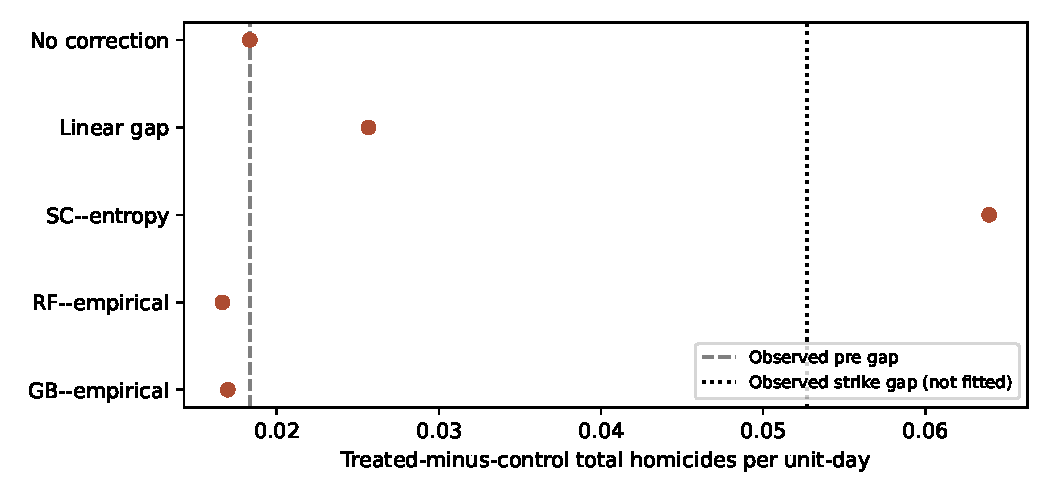
\includegraphics[width=0.83\linewidth]{figures/empirical_counterfactual_gap_rebuild.pdf}
\caption{Total-homicide untreated strike-gap forecasts. The observed strike gap is displayed only for comparison and is excluded from every candidate's fit and from the pre-strike selection.}\label{fig:counterfactualrebuild}
\end{figure}

\subsection{External comparison and sensitivity}
The released Mancha specification regresses the nonzero-observation unit--day outcome on a statewide strike indicator and its interaction with high gang exposure, absorbing municipality/district, AIS--year, month and weekday effects. It uses the 2014--2020 source sample rather than the balanced 97-day main window; in our replication it has 21,886 source unit--day observations after the original singleton/duplicate handling. Its interaction is not the unit/date TWFE DID in Equation~\ref{eq:empiricaltwfe}: zero-filled days, date effects, sample duration, implicit observation weights and, for the published code, treatment coding all differ. With the executed four-AIS coding, the reproduced total-homicide interaction is 0.334996, matching the published 0.335 after rounding. Six other reproduced interactions are within 0.0006 of the printed coefficients; the largest discrepancy is for women (0.068401 versus published 0.069), which is not identical at three-decimal rounding and remains unresolved. Correcting that \emph{same} external specification to five AIS gives 0.224398. Neither coefficient is inserted into Equation~\ref{eq:empiricalbias}; the difference from this thesis's 0.03437 TWFE is not an estimate of ``bias corrected away.''

\begin{table}[htbp]
\centering\small
\caption{External replication of Mancha's interaction regression versus this thesis's distinct TWFE benchmark. Coefficients are not subtracted from one another.}
\label{tab:mancharebuild}
\begin{tabular}{lrrrr}
\toprule
Outcome & Published & Replicated four AIS & Corrected five AIS & Thesis TWFE\\
\midrule
Total & 0.335 & 0.335 & 0.224 & 0.034\\
Men & 0.267 & 0.267 & 0.184 & 0.032\\
Women & 0.069 & 0.068 & 0.040 & 0.002\\
Crime 1 & 0.297 & 0.297 & 0.236 & 0.021\\
Crime 2 & 0.267 & 0.267 & 0.188 & 0.018\\
Crime 3 & 0.180 & 0.180 & 0.083 & 0.012\\
Crime 4 & 0.159 & 0.159 & 0.060 & 0.009\\
\bottomrule
\end{tabular}
\end{table}


Table~\ref{tab:sensitivityrebuild} changes the pre-period from 8 to 104 weeks, applies the executed four-AIS and mechanical six-AIS definitions, and aggregates at AIS--day rather than municipality/district--day. Four-AIS coding increases the 12-week TWFE to about 0.0568; adding AIS 07 produces about 0.0349. The AIS aggregate estimates are on a different count scale and weight AIS equally instead of municipalities. Synthetic Control's negative main-window result is sensitive to horizon, becoming slightly positive at 104 weeks. These contrasts show that treatment definition, forecast support and analysis unit matter; they are not alternative measurements of a known ATT.

\begin{longtable}{lrrrrr}
\caption{Total-homicide sensitivity to pre-period length, treatment definition, and aggregation. Entries are adjusted estimates, not comparable across the last unit-aggregation row in absolute scale.}\label{tab:sensitivityrebuild}\\
\toprule
Specification & TWFE & Linear & SC & RF & GB\\
\midrule
Five AIS, 8 weeks & 0.032 & 0.027 & -0.011 & 0.037 & 0.036\\
Five AIS, 12 weeks & 0.034 & 0.027 & -0.011 & 0.036 & 0.036\\
Five AIS, 26 weeks & 0.037 & 0.031 & -0.011 & 0.036 & 0.036\\
Five AIS, 52 weeks & 0.038 & 0.036 & -0.011 & 0.035 & 0.036\\
Five AIS, 104 weeks & 0.037 & 0.038 & 0.003 & 0.035 & 0.034\\
Four AIS, 12 weeks & 0.057 & 0.050 & 0.008 & 0.061 & 0.061\\
Six AIS, 12 weeks & 0.035 & 0.029 & -0.019 & 0.038 & 0.037\\
AIS--day, 12 weeks & 0.767 & 0.619 & -0.754 & 0.790 & 0.785\\
\bottomrule
\end{longtable}


{\footnotesize\begin{longtable}{llrrrrrr}
\caption{All-outcome pre-strike placebo performance (same 154 windows and models in each row).}\label{tab:allplaceborebuild}\\
\toprule
Outcome & Method & Signed error & Variance & MAE & RMSE & Windows & Failures\\
\midrule
\endfirsthead
\toprule
Outcome & Method & Signed error & Variance & MAE & RMSE & Windows & Failures\\
\midrule
\endhead
Total & No correction & 0.00028 & 0.000069 & 0.00675 & 0.00830 & 154 & 0\\
Total & Linear gap & -0.00008 & 0.000090 & 0.00755 & 0.00946 & 154 & 0\\
Total & SC--entropy & 0.00105 & 0.000076 & 0.00718 & 0.00876 & 154 & 0\\
Total & RF--empirical & 0.00202 & 0.000061 & 0.00642 & 0.00809 & 154 & 0\\
Total & GB--empirical & 0.00018 & 0.000067 & 0.00655 & 0.00820 & 154 & 0\\
\midrule
Men & No correction & 0.00027 & 0.000060 & 0.00630 & 0.00775 & 154 & 0\\
Men & Linear gap & -0.00005 & 0.000082 & 0.00703 & 0.00904 & 154 & 0\\
Men & SC--entropy & 0.00102 & 0.000069 & 0.00682 & 0.00840 & 154 & 0\\
Men & RF--empirical & 0.00183 & 0.000055 & 0.00597 & 0.00767 & 154 & 0\\
Men & GB--empirical & 0.00020 & 0.000063 & 0.00620 & 0.00793 & 154 & 0\\
\midrule
Women & No correction & 0.00001 & 0.000004 & 0.00140 & 0.00188 & 154 & 0\\
Women & Linear gap & -0.00003 & 0.000005 & 0.00171 & 0.00216 & 154 & 0\\
Women & SC--entropy & 0.00034 & 0.000004 & 0.00148 & 0.00191 & 154 & 0\\
Women & RF--empirical & 0.00033 & 0.000003 & 0.00138 & 0.00183 & 154 & 0\\
Women & GB--empirical & 0.00004 & 0.000004 & 0.00154 & 0.00192 & 154 & 0\\
\midrule
Crime 1 & No correction & 0.00006 & 0.000030 & 0.00446 & 0.00544 & 154 & 0\\
Crime 1 & Linear gap & -0.00016 & 0.000037 & 0.00479 & 0.00610 & 154 & 0\\
Crime 1 & SC--entropy & 0.00057 & 0.000033 & 0.00463 & 0.00579 & 154 & 0\\
Crime 1 & RF--empirical & 0.00102 & 0.000028 & 0.00433 & 0.00538 & 154 & 0\\
Crime 1 & GB--empirical & 0.00003 & 0.000032 & 0.00450 & 0.00563 & 154 & 0\\
\midrule
Crime 2 & No correction & 0.00006 & 0.000025 & 0.00411 & 0.00497 & 154 & 0\\
Crime 2 & Linear gap & -0.00015 & 0.000031 & 0.00439 & 0.00559 & 154 & 0\\
Crime 2 & SC--entropy & 0.00056 & 0.000027 & 0.00423 & 0.00522 & 154 & 0\\
Crime 2 & RF--empirical & 0.00098 & 0.000022 & 0.00394 & 0.00483 & 154 & 0\\
Crime 2 & GB--empirical & 0.00007 & 0.000027 & 0.00413 & 0.00517 & 154 & 0\\
\midrule
Crime 3 & No correction & 0.00006 & 0.000019 & 0.00352 & 0.00439 & 154 & 0\\
Crime 3 & Linear gap & -0.00014 & 0.000025 & 0.00406 & 0.00504 & 154 & 0\\
Crime 3 & SC--entropy & 0.00056 & 0.000020 & 0.00357 & 0.00449 & 154 & 0\\
Crime 3 & RF--empirical & 0.00086 & 0.000018 & 0.00337 & 0.00428 & 154 & 0\\
Crime 3 & GB--empirical & 0.00003 & 0.000021 & 0.00363 & 0.00455 & 154 & 0\\
\midrule
Crime 4 & No correction & 0.00008 & 0.000016 & 0.00318 & 0.00402 & 154 & 0\\
Crime 4 & Linear gap & -0.00005 & 0.000022 & 0.00378 & 0.00474 & 154 & 0\\
Crime 4 & SC--entropy & 0.00056 & 0.000016 & 0.00324 & 0.00408 & 154 & 0\\
Crime 4 & RF--empirical & 0.00084 & 0.000016 & 0.00325 & 0.00413 & 154 & 0\\
Crime 4 & GB--empirical & 0.00011 & 0.000020 & 0.00350 & 0.00445 & 154 & 0\\
\bottomrule
\end{longtable}
}

\section{Discussion}\label{sec:discussion}
The simulation isolates the correction's mechanism: when the untreated gap's functional form is known, a matching forecast can largely remove its induced DID bias. Yet reducing signed bias can increase variance, so RMSE improves only when the avoided bias is large relative to extrapolation noise. That is an oracle result because the simulation knows the true functional form and ATT. The empirical study cannot observe either and therefore substitutes pre-strike out-of-sample pseudo-effects for model selection, not for direct estimation of true ATT bias.

The expanded Cear\'a comparison demonstrates why that distinction matters. The forest's slight pre-strike RMSE advantage selects it for total homicides in the original sample, but its strike adjustment is small and in the opposite direction from the linear and Synthetic Control adjustments. The full re-selection bootstrap instead chooses no correction in 61 of 99 draws and the forest in only 15, with Synthetic Control in 19 and boosting in four. This is direct evidence that the narrow pre-strike ranking is sensitive to AIS composition, not evidence about the unobserved strike counterfactual. The five candidates share one TWFE baseline and the same unit weights; differences arise from their forecasts of the missing untreated gap, not from substituting a published coefficient. The forest's win is not a universal algorithm ranking: its covariates had to be redefined because simulated $X_1,X_2,X_3$ were unavailable. Synthetic Control's use of contemporaneous donor outcomes is a different, potentially valuable information set, but the one-predictor matching design does not guarantee a credible post-strike untreated path.

Rolling placebo performance provides a disciplined comparison under historical no-treatment conditions. It does not establish that an unobserved untreated gap during a police strike would continue to obey the same relationship. Nor should overlapping training windows be interpreted as 154 independent experiments. The AIS bootstrap and selection-aware re-estimation address sampling and model-selection variation within the observed cluster structure, but five treated clusters leave wide scope for finite-cluster error and sensitivity to the composition of the treated arm. Sex classification, the ambiguous AIS 07 cutoff, and differences between the published and executed treatment code are additional measurement and design constraints.

The practical lesson is to state the estimating object before attempting a correction, align every forecast to its pre-period baseline and weights, pre-specify a no-correction candidate, select only with untreated pre-period evidence, and report the whole candidate set together with external estimands clearly separated. Such a workflow permits an adjustment without pretending that predictive validation identifies a missing causal counterfactual. Further work could compare longer-horizon validation, regularized forecasts, and inference designed specifically for very few treated clusters.

\section{Conclusion}\label{sec:conclusion}
This thesis evaluates a transparent DID bias correction: predict the untreated treated--control gap during treatment, subtract its change from the same pre-treatment gap embedded in TWFE, and keep that benchmark common to all methods. In the controlled simulation, a correctly specified correction can nearly eliminate average bias, but lower RMSE is conditional on a sufficiently strong violation. In the Cear\'a application, the original-sample pre-strike RMSE rule selects Random Forest for total homicides and five other outcomes, while retaining unadjusted TWFE for one. The selected total-homicide point estimate is close to TWFE, its pre-strike RMSE improvement is modest, and complete AIS resampling often selects a different method. The selected-procedure total-homicide interval includes zero. The substantive conclusion must therefore remain cautious: these calculations compare historically predictive counterfactual procedures, not directly observed strike-period ATT bias. The value of the framework is its auditable link between estimand, forecast, validation, uncertainty and sensitivity, rather than a claim that one adjustment always dominates.
